\section{HJSON Web Framework}\label{hjson-web-framework}

The HIJSON Web Framework responds to the needs of an extendable,
customizable, and scalable web framework which provides at the same time IoT
monitoring, realtime multi-person tracking and crossfloor user
navigation.

Expandability and customizability derives from both design choises and
HIJSON inherent characteristics, the possibility of semantic extensions.
Scalablility is directly borrowed from technologies used for the
software development: \emph{JavaScript} language, using \emph{Node.js},
in particular \emph{Express.js} as backend framework, exploiting the
power of WebSocket protocol through the \emph{Socket.io} library.

Being supported by the web as bearing platform, the framework exposes
also an highly availability: it is so simple to use as to visit a
website, both from desktop or mobile devices, without explicit
requirements to install any software from proprietary stores (access to
which is often denied from business devices).

The HIJSON Web Framework deeply relies on HIJSON Toolkit and offers the
overal client/server architecture and a convinient, highly intractive
user interface, leaving aside the specific indoor positioning system and
the IoT sensors, to deal with a robust interface is provided and
described in the following seciton.

\subsection{Applications}\label{applications}

The Framework has been designed focus on two different possible kind of
users: the \emph{Explorer} and the \emph{Supervisor}. They have
different requirements and are likely equipped with different devices:
while the \emph{Supervisor} monitors the indoor environment through a
desktop workstation, the \emph{Explorer} has a smartphone available and
needs to be routed across the building.

In both cases, the web platform ensures a perfect alignment with the
BYOD (Bring Your Own Device) approach, nowadays often supported by companies
that encourage employees to use personal devices.

\begin{figure*}[htb]
\centering
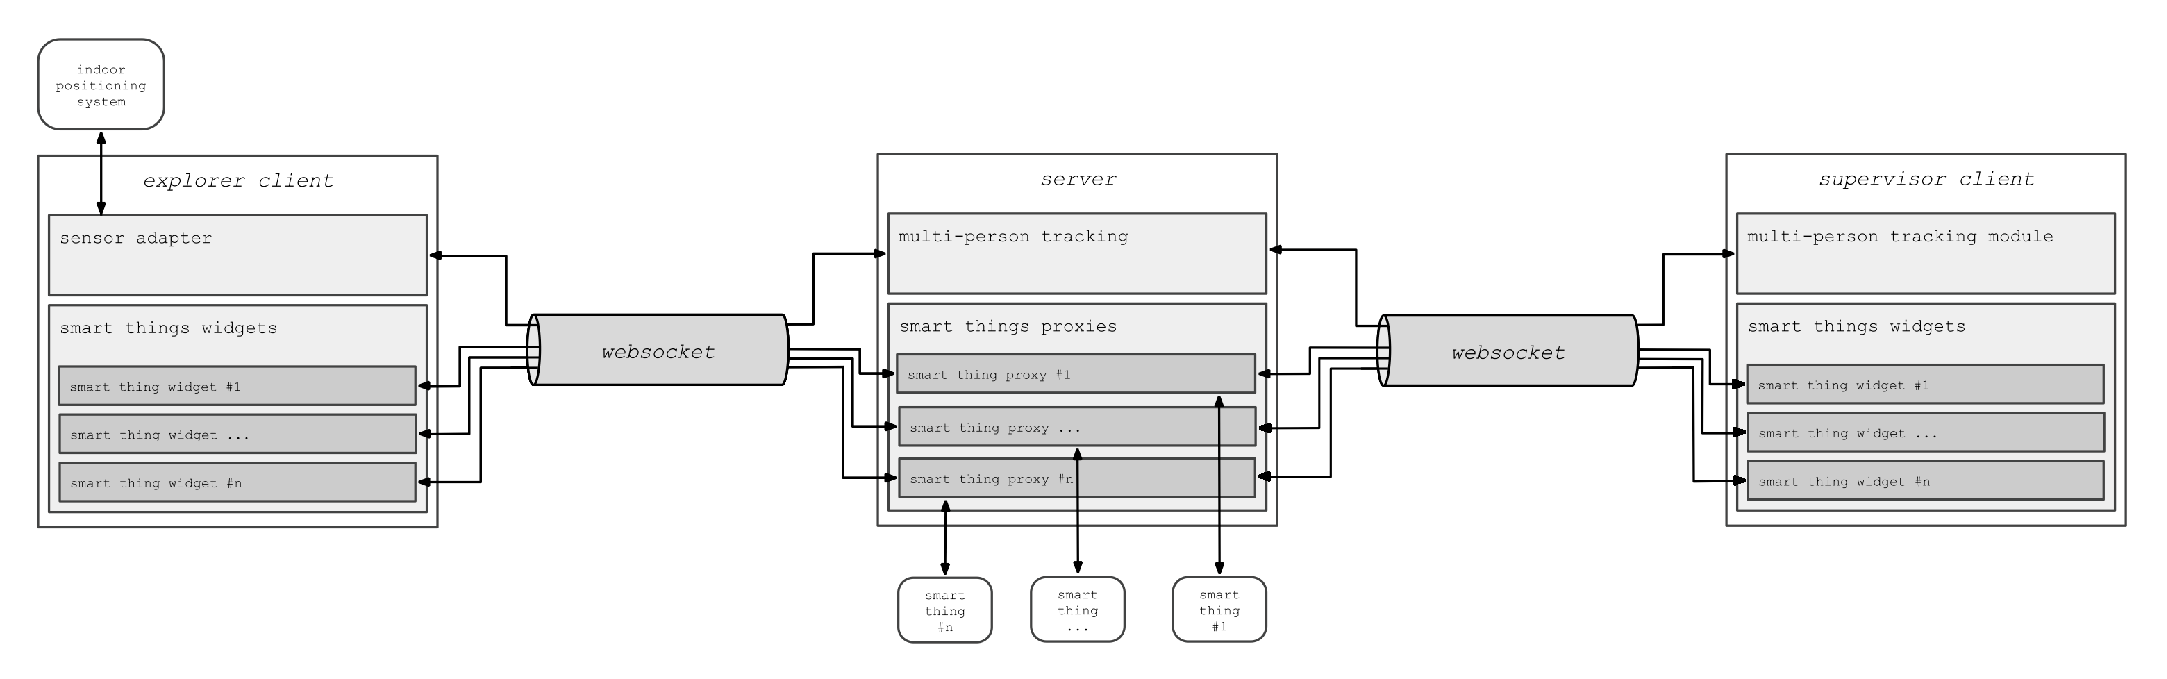
\epsfig{file=images/architecture.eps, width=\textwidth}
\caption{HIJSON Web Toolkit architecture}
\label{fig:architecture}
\end{figure*}


\subsubsection{IoT monitoring}\label{iot-monitoring}

Every element in the HIJSON environment is capable of showing information
about itself, so it can be analyzed by the user. The modularity of the HIJSON
Toolkit permits to show particular information or UI about a specific object,
using polymorphic behaviours of the different HIJSON Nodes. If an object is
connected to the network and it is capable of interaction, the user can
benefit of its functions through the system (e.g. if the object is a
thermostat, the user can see the temperature in the room and can turn on/off
the heating). If the object isn't interactive, the system can show static
information (e.g. for fire Extinguisher, the system shows the last date of
checking).

\subsubsection{Realtime multi-person tracking}\label{realtime-multi-person-tracking}

A typical task performed by a \emph{Supervisor} can be the monitoring of users
locations inside the building. This operation can be required for various
reasons, e.g. security or logistics. The devices that equips the
\emph{Explorers} can be used to track their position in realtime, giving the
\emph{Supervisors} the whole picture of the presences inside the building in
every moment.

\subsubsection{Cross-storey user navigation}\label{cross-storey-user-navigation}

As shown in the algorithmics section, the HIJSON Toolkit provides a particular
strategy to assemlbe a graph of possible paths inside the building. This
graph, represented also in the form of a weighted adjacency matrix, can be
easely used to compute paths between two nodes inside the building. To
achieve this result, the matrix, which edges are weighted according to the
distance between two nodes, is used as input in an applicaiton of the
Dijkstra's algorithm. The result is the shortest path between two selected
nodes of the graph. Thanks to the cross-storey connections of nodes
representing stairs or elevators, the paths calculated can also start and end
on different stories.



\subsection{Architecture}\label{architecture}

Like the vast majority of the web based application, the Framework exposes an
overall architecture that is inherently \emph{client/server}. In particular,
two different type of possible client are identifiable, one for each different 
kind of users: the \emph{Supervisor} client and the \emph{Explorer} client. 
Both of them connect to the same server.

The indoor space described by the HIJSON document passed as input is
processed by the server via the processing pipeline. After that any connecting
\emph{Explorer} client, presumably through a mobile device, will be provided
with the information to perform cross-storey navigation of the building, while
reporting user position to the server. The server will feed any connecting
\emph{Supervisor} client with users positions, along with data from sensor-
equipped objects present in the environment, realizing the IoT monitoring and
the realtime multi-person tracking.

\subsubsection{Server Architecture}\label{server-architecture}

The complete architectural scheme of the framework is provided in figure
\ref{fig:architecture}. A web server module is responsible for listenning to
connecting clients. Each client connection is handled by the web server module
providing all the required resources and opening one websocket channel,
through which will flow \emph{Explorer} and/or \emph{Supervisor} communication
protocol data. In particular, {\tt multi-person\ tracking} module receives
position data from \emph{Explorer} clients. It aggregates and sends these
information to connected \emph{Supervisor} clients through the websocket
channel, using a simple but realible protocol described later. Indipendence
from particular IoT sensor equipment communication protocol is achieved
introducing one {\tt smart\ object\ proxy} module (defined in the HIJSON Class
and obtained with {\tt getProxy} method previously described) for each smart
object modelled.

\subsubsection{Explorer client architecture}\label{explorer-client-architecture}

The \emph{Explorer} client architecture is generally deployed on a mobile
device, which is usually supplied to a user who needs to be routed across the
environment described by HIJSON document. The {\tt sensor\ adapter} module
encapsulates the communication logic with the indoor positioning system. The
presence of this module ensures indipendece from particularly tecnology
allowing client \emph{Explorer} to rely on different indoor positioning
systems (WiFi, LTE, etc.).

Every time the {\tt sensor\ adapter} observe a perceptible
modification in user position sends the new position information to the
server through the single opened websocket, using the a message with the
following syntax:

\begin{verbatim}
currentPosition = {
 coordinates: [x, y],
 levelId: level-ID 
}
\end{verbatim}

Relevant information includes, beside current coordinates, the indication of
the storey of the possibly multilevel building the user is in.

It is to remark that, when not outflanked by the introduction of an external
server, the problem of communication between positioning system and the low
level APIs of the browser is left to positioning system itself or to whom is
in charge of specific deployments of the HIJSON Web Framework.

The {\tt smart\ object\ widget} module, being in common with the
client \emph{Supervisor}, has been treated in the next section.

\subsubsection{Supervisor client architecture}\label{supervisor-client-architecture}

The Client \emph{Supervisor} architecture shows two modules. The first
one, the {\tt multi-person\ tracking} module, is responsible to
receive through the websocket, from the server information about
explorers of the environment, showing them in the user interface. The
second module, the {\tt smart\ object\ widget} communicates with the
server to propose to the user realtime information about sensor-equipped
objects in the environment. Data passes through the single websocket
opened between the server and every \emph{Supervisor} Client. Rely on a
naive but effective communication protocol, each {\tt smart object widget}
exchange data only with respective {\tt smart pbject proxy} on the server. To
ensure the the data is sent only when the user requires the information
relative to a specific smart object, a widget lifecycle protocol is
implemented: it is based on the 4 events {\tt on\_before\_show},
{\tt on\_show}, {\tt on\_before\_hide}, {\tt on\_hide}
triggered, as suggested by their names when a widget is shown or hidden.
When the user requires information about a smart object, its widget has
to be rendered, but {\tt on\_before\_show} the server is notified to
connect via relative proxy to the sensor. Once connected, the server
begin to send data via webscocket. Received data is shown through the
wodget to the user. When done, that is the {\tt on\_before\_hide} event of the
widget is triggered, a notification is sent to the server announcing to stop sending
data and the proxy close the connection to the sensor. Widget lifecycle
protocol ensures that only requiring data is sent from th eserver to the
client.
